\section{Dependence on the Architecture of the NTK}
\label{sec:NTKArchDep}

It is interesting to consider what happens to the picture sketched so far as the
architecture of the neural networks is varied. In Fig.~\ref{fig:NTKTimeDiffArch}
we compare the time dependence of the Frobenius norm of the NTK and the
variation of the first three eigenvalues for two different architectures. The
smaller network is the $[28,20]$ used in the standard NNPDF analyses and in this
work, while the large one is a $[100,100]$ network, which is closer to the
infinite-width limit. For illustration purposes we focus in this plot on L1 data
and only three eigenvalues rather than the five we examined above. The
quantitative features are exactly the same for L0 and L2 data, and adding the
fourth and fifth eigenvalues does not add unexpected behaviours compared to what
we observe in Fig.~\ref{fig:NTKTime}. It is interesting to remark that the onset
of lazy training is slower for the larger network. This is to be expected if we
interpret the early stages of training as a phase where the network identifies
the learnable features in the space of functions that it can parametrize. For a
larger network, the space of parametrized functions is larger and the
identification of the physical features takes a larger number of epochs. 
% ===================================
\begin{figure}[t]
  \centering
  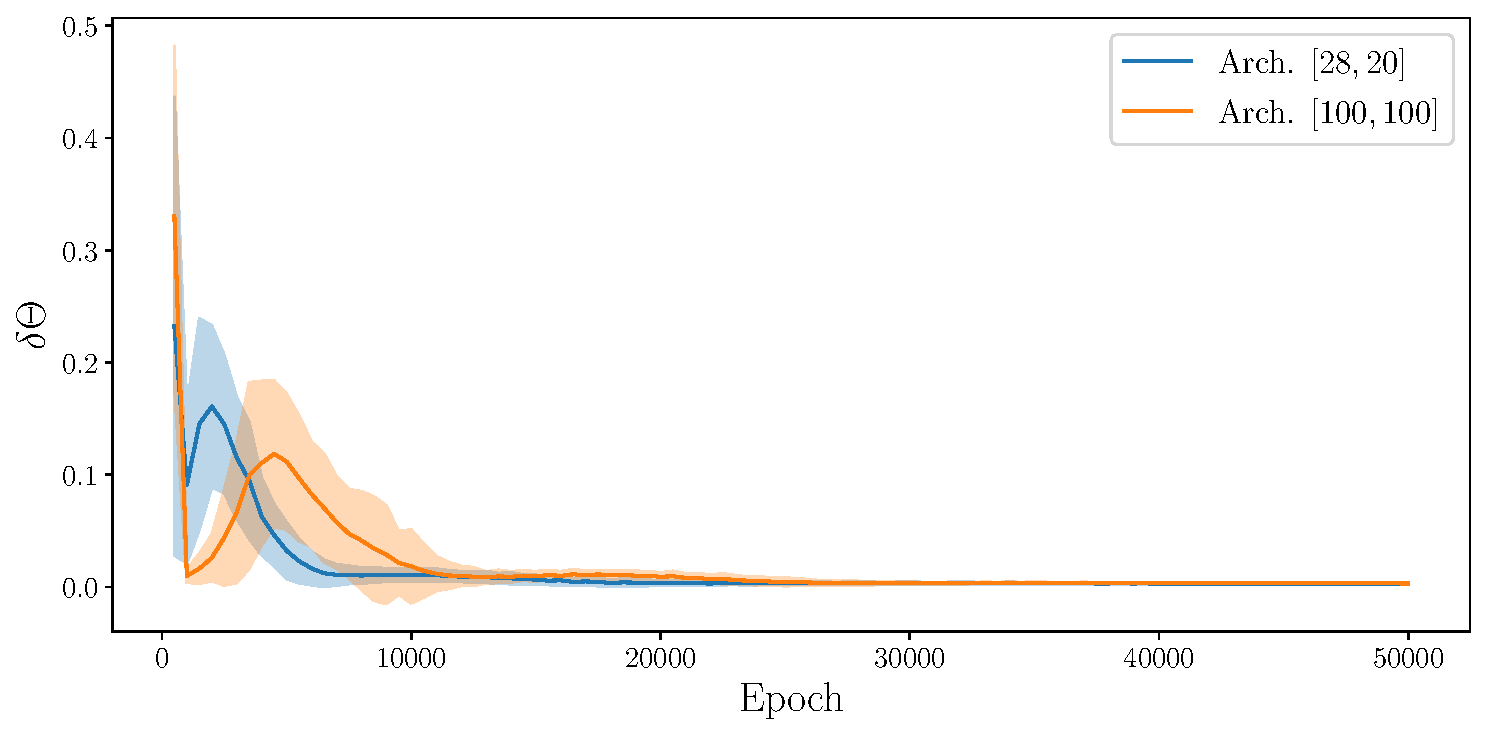
\includegraphics[width=0.45\textwidth]{appendix_arch/delta_ntk_arch.pdf}
  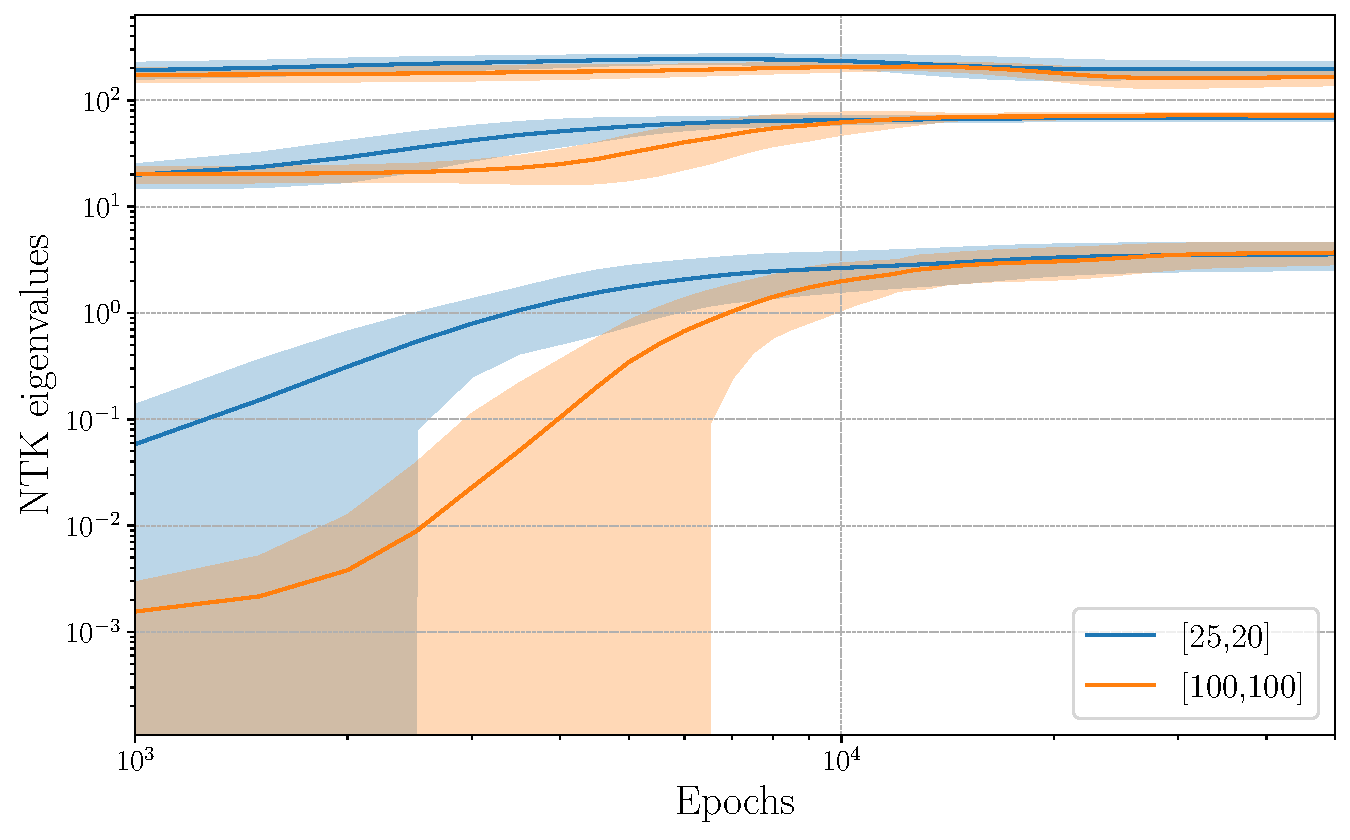
\includegraphics[width=0.45\textwidth]{appendix_arch/ntk_eigvals_single_plot_arch.pdf}
  \caption{Comparison of the variation of the NTK during training (left) and the
  first three eigenvalues (right) for two different architectures with sizes
  $[28,20]$ and $[100,100]$ respectively. In both cases, L0 data is used. In the
  left plot, error bands represent the standard deviation over the ensemble of
  replicas. In the right plot, solid lines represent the median over the
  ensemble of networks, while solid bands correspond to 68\% confidence level.}
  \label{fig:NTKTimeDiffArch}
\end{figure}
% ===================================

\FloatBarrier